\section{Equilibrios modelo}

\begin{framed}
\noindent Sean $\gamma_j$ la estrategia del jugador $j$, $k \in \{f,m\}$,  $\theta^e$ el costo esperado por el jugador 2 de que el jugador 1 esté violando la norma social, y $\hat{\theta}^e$ el costo esperado por el jugador 2 fuera de la senda de equilibrio de que el jugador 1 esté violando la norma social,

\noindent (i) $(\gamma_1(k)=\gamma_1(-k)=\gamma_1(o)=E_k, \gamma_2(E_k)=i, \gamma_2(E_{-k})=i)$ es equilibrio si $\eta\in[\theta^e, \infty) \wedge \eta\in[\hat{\theta}^e, \infty) \wedge \Pi_1(E_{k})- \xi \geq \Pi_1(E_{-k})$

\noindent (ii) $(\gamma_1(k)=\gamma_1(-k)=\gamma_1(o)=E_k, \gamma_2(E_k)=i, \gamma_2(E_{-k})=ni)$ es equilibrio si $\eta\in[\theta^e, \infty) \wedge \eta\in (0, \hat{\theta}^e) \wedge \Pi_1(E_{k})- \xi \geq \Pi_1(E_{-k}-\beta)$

\noindent (iii) $(\gamma_1(k)=\gamma_1(-k)=\gamma_1(o)=E_k, \gamma_2(E_k)=ni, \gamma_2(E_{-k})=i)$ es equilibrio si $\eta\in (0, \theta^e) \wedge \eta\in[\hat{\theta}^e, \infty) \wedge \Pi_1(E_{k})- \xi -\beta \geq \Pi_1(E_{-k})$

\noindent (iv) $(\gamma_1(k)=\gamma_1(-k)=\gamma_1(o)=E_k, \gamma_2(E_k)=ni, \gamma_2(E_{-k})=ni)$ es equilibrio si $\eta\in (0, \theta^e) \wedge \eta\in(0, \hat{\theta}^e) \wedge \Pi_1(E_{k})- \xi \geq \Pi_1(E_{-k})$
\end{framed}

\begin{figure}
\caption{Equilibrios agrupadores}
\hspace*{-2cm}
\begin{minipage}{0.49\textwidth}
    \centering
    Si $\theta^e > \hat{\theta}^e$
    
    \scriptsize{
    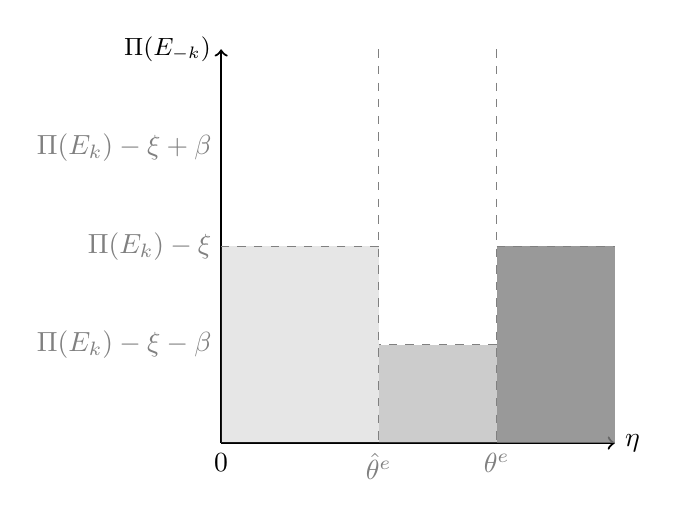
\begin{tikzpicture}
         \draw[black, thick][->] (0,0) -- (5,0) node[right] {$\eta$};
         \draw[black, thick][->] (0,0) node[below]{0} -- (0,5) node[left] {\small{$\Pi(E_{-k})$}};
         \draw[gray, dashed] (2,5) -- (2,0) node[below] {$\hat{\theta}^e$};
         \draw[gray, dashed] (3.5,5) -- (3.5,0) node[below] {$\theta^e$};
         
         \draw[gray, dashed] (3.5,1.25) -- (2,1.25);
         \draw[gray] (0, 1.25) node[left] {$\Pi(E_k)-\xi-\beta$};
         
         \draw[gray, dashed] (3.5, 2.5) -- (5,2.5) (2,2.5) -- (0,2.5) node[left] {$\Pi(E_k)-\xi$};
         
         \draw[gray] (0,3.75) node[left] {$\Pi(E_k)-\xi+\beta$};
         \draw[draw=gray, draw opacity=0, fill=gray, fill opacity=0.2] (2,0)--(0,0)--(0,2.5)--(2,2.5) -- cycle;
         
         \draw[draw=gray, draw opacity=0, fill=gray, fill opacity=0.4] (2,0)--(3.5,0)--(3.5,1.25)--(2,1.25) -- cycle;
         
         \draw[draw=gray, draw opacity=0, fill=gray, fill opacity=0.8] (5,0)--(3.5,0)--(3.5,2.5)--(5,2.5) -- cycle;
    \end{tikzpicture}}
\end{minipage}
\begin{minipage}{0.49\textwidth}
\centering
    Si $\theta^e < \hat{\theta}^e$

    \scriptsize{
    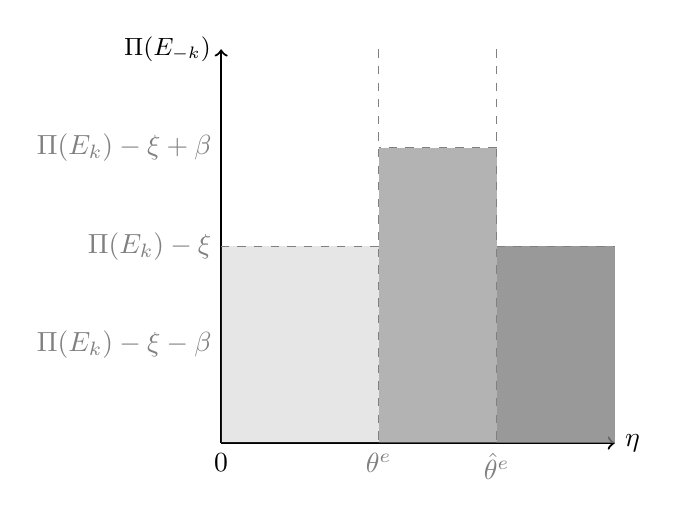
\begin{tikzpicture}
         \draw[black, thick][->] (0,0) -- (5,0) node[right] {$\eta$};
         \draw[black, thick][->] (0,0) node[below]{0} -- (0,5) node[left] {\small{$\Pi(E_{-k})$}};
         \draw[gray, dashed] (2,5) -- (2,0) node[below] {$\theta^e$};
         \draw[gray, dashed] (3.5,5) -- (3.5,0) node[below] {$\hat{\theta}^e$};
         
         \draw[gray, dashed] (3.5, 3.75) -- (2,3.75) ;
         \draw[gray] (0, 1.25) node[left] {$\Pi(E_k)-\xi-\beta$};
         
         \draw[gray, dashed] (3.5, 2.5) -- (5,2.5) (2,2.5) -- (0,2.5) node[left] {$\Pi(E_k)-\xi$};
         
         \draw[gray] (0,3.75) node[left] {$\Pi(E_k)-\xi+\beta$};
         \draw[draw=gray, draw opacity=0, fill=gray, fill opacity=0.2] (2,0)--(0,0)--(0,2.5)--(2,2.5) -- cycle;
         
         \draw[draw=gray, draw opacity=0, fill=gray, fill opacity=0.6] (2,0)--(3.5,0)--(3.5,3.75)--(2,3.75) -- cycle;
         
         \draw[draw=gray, draw opacity=0, fill=gray, fill opacity=0.8] (5,0)--(3.5,0)--(3.5,2.5)--(5,2.5) -- cycle;
    \end{tikzpicture}}
\end{minipage}
\begin{minipage}{\textwidth}
    \centering
    \vspace*{0.5cm}
    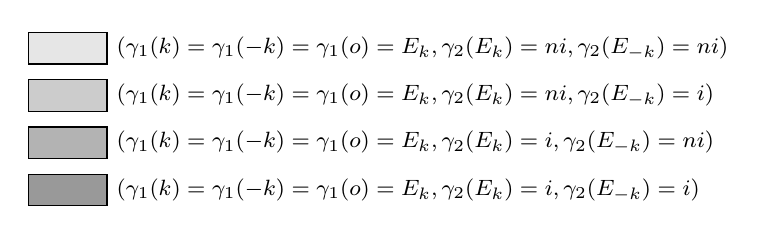
\begin{tikzpicture}
         \draw[draw=black, draw opacity=1, fill=gray, fill opacity=0.2] (1,1.8)--(0,1.8)--(0,2.2)--(1,2.2) -- cycle;
         \draw[black] (1,2) node[right] {\footnotesize{$(\gamma_1(k)=\gamma_1(-k)=\gamma_1(o)=E_k, \gamma_2(E_k)=ni, \gamma_2(E_{-k})=ni)$}};
         
         \draw[draw=black, draw opacity=1, fill=gray, fill opacity=0.4] (1,1.2)--(0,1.2)--(0,1.6)--(1,1.6) -- cycle;
         \draw[black] (1,1.4) node[right] {\footnotesize{$(\gamma_1(k)=\gamma_1(-k)=\gamma_1(o)=E_k, \gamma_2(E_k)=ni, \gamma_2(E_{-k})=i)$}};
         
         \draw[draw=black, draw opacity=1, fill=gray, fill opacity=0.6] (1,0.6)--(0,0.6)--(0,1)--(1,1) -- cycle;
         \draw[black] (1,0.8) node[right] {\footnotesize{$(\gamma_1(k)=\gamma_1(-k)=\gamma_1(o)=E_k, \gamma_2(E_k)=i, \gamma_2(E_{-k})=ni)$}};
         
         \draw[draw=black, draw opacity=1, fill=gray, fill opacity=0.8] (1,0)--(0,0)--(0,0.4)--(1,0.4) -- cycle;
         \draw[black] (1,0.2) node[right] {\footnotesize{$(\gamma_1(k)=\gamma_1(-k)=\gamma_1(o)=E_k, \gamma_2(E_k)=i, \gamma_2(E_{-k})=i)$}};
         
    \end{tikzpicture}
\end{minipage}
\begin{singlespace}
    \floatfoot{\footnotesize{\textit{Nota:} La figura representa los equilibrios agrupadores del modelo. $\beta$ es el costo que percibe el jugador 1 de no interactuar con el jugador 2. $\xi$ es el costo de violar uno mismo la norma social. $\eta$ es el costo que percibe el jugador 2 de no interactuar con el jugador 1, $\theta^e$ es el costo esperado por el jugador 2 de que el jugador 1 esté violando la norma social y $\hat{\theta}^e$ el costo esperado por el jugador 2 fuera de la senda de equilibrio de que el jugador 1 esté violando la norma social.}\par}
\end{singlespace}

\label{fig:equilibriosagru}
\end{figure}




